\chapter{Proposta}

A seguir será detalhado cada ponto proposto neste trabalho em tópicos mais específicos.

\section{O Framework}

A proposta deste trabalho é desenvolver um framework que auxilie no desenvolvimento de redes sociais. Este framework deve oferecer recursos gerais como toda a lógica de usuários e relacionamentos e recursos de rotas e agendas. O recurso de rotas deve ser capaz de fazer um mapeamento de trajetos de interesse de um determinado usuário e auxiliar este a fazer comparações com rotas de outros usuários. A agenda deve oferecer recursos de controle de ocupações no decorrer de dias e horários e auxiliar um usuário a encontrar dias e/ou horários comuns entre um grupo de usuários qualquer.

\subsection{Relacionamento de Usuários}

O relacionamento em redes sociais dá-se por meio de iterações entre os usuários, estas iterações variam de acordo com a rede em que o usuário está inserido. Alguém pode apenas seguir outras pessoas e acompanhar suas postagens, este é um relacionamento unidirecional, pois não é nessário que uma pessoa seguida acompanhe também postagens de seus seguidores. Existe também outro tipo de relacionamento onde é necessário que as duas pessoas estejam diretamente ligadas entre si, o que o torna necessariamente bidirecional, neste tipo pode-se considerar relacionamentos entre conhecidos, amigos, namorados, familiares, entre outros.

Na montagem da estrutura de relacionamentos entre os usuários para redes sociais é nessário fazer uso de grafos onde os usuários serão representados como os vértices e os relacionamentos como as arestas. No caso dos relacionamentos unidirecionais apenas uma aresta é criada. Esta aresta faz uma ligação a partir do vértice do usuário seguidor para o vértice do usuário que este deseja seguir. No caso dos relacionamentos bidirecionais a ligação deverá ser feita usando-se duas arestas paralelas. É necessário que ambos os usuários exista uma possibilidade de se chegar ao outro, portanto, deve existir uma aresta que ligue um usuário ``A'' a um usuário ``B'' e uma aresta que ligue o usuário ``B'' ao usuário ``A''.

Cada aresta deverá possuir uma ou mais descrições que detalham qual o relacionamento entre os usuários. Isso fica mais claro ao se falar de relacionamentos bidirecionais, onde pode existir entre duas pessoas um relaciomanento de amizade e parentesco, por exemplo.

A seguir têm-se algumas imagens que exemplificam os relacionamentos citados.

% A -> B
% C -> B

% 	amigo
% A <-> B

% 	amigo
% 	mae
% 	filho
% A <-> B

\subsection{Controle de Rotas}

Rota\footnote{\url{http://www.dicio.com.br/rota/}} é um itenerário que se percorre para ir de um lugar a outro, indicando a direção ou rumo a ser percorrido, um exemplo de rota pode ser visualizado na figura \ref{rota}.

\begin{figure}[!h]
	\centering
	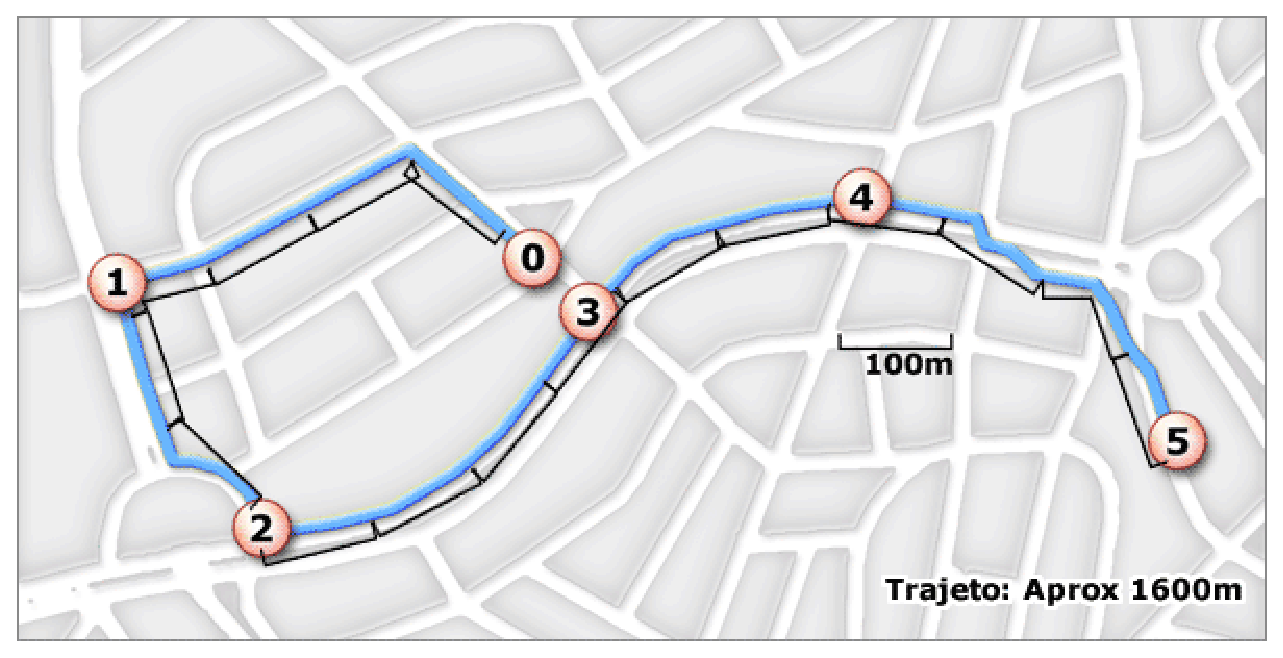
\includegraphics[scale=0.55]{figuras/capitulo5/rota.eps}
	\caption{Exemplo de rota}
	\label{rota}
\end{figure}

O framework irá oferecer recursos que auxiliem o usuário a definir as rotas que percorre e os horários de cada percurso e buscar rotas de outros usuários que coincidem em parte ou integralmente com as suas.

Redes socias podem utilizar estes dados para aplicações diversas como, por exemplo, caronas e encontros para ciclistas.

\subsection{Controle de Agenda}

Outra funcionalidade que o framework irá fornercer é a conciliação de agendas entre os usuários, possibilitando assim encontrar dias da semana e horários específicos que são comuns a um determinado grupo. Esta funcinalidade pode auxiliar os usuários em diversos aspectos como, por exemplo, encontrar um horário em comum para realizar uma tarefa.

\section{Uso do Framework}

O framework será desenvolvido em \textit{``Ruby on Rails''} e terá sua \textit{``Gem''}\footnote{\url{http://www.akitaonrails.com/2009/2/2/entendendo-rubygems}} publicada em um repositório online para uso de outros desenvolvedores.

Para comprovação do funcionamento do framework, este trabalho propõe o desenvolvimento de uma rede social que faça uso do mesmo. Esta rede deverá fazer uso dos principais recursos providos pelo framework, dessa forma, pode-se ver o seu uso na prática.

\section{Prova de Conceito}

\subsection{Algoritmos}

\subsection{Modelo Inicial}

Como apresentado na figura \ref{diagrama de classe} o modelo de classes possui as classes de usuário, grupo, rota e agenda. No qual, um usuário pode pertencer muitos grupos, pode ter uma agenda e pode possuir muitas rotas.

\begin{figure}[!h]
	\centering
	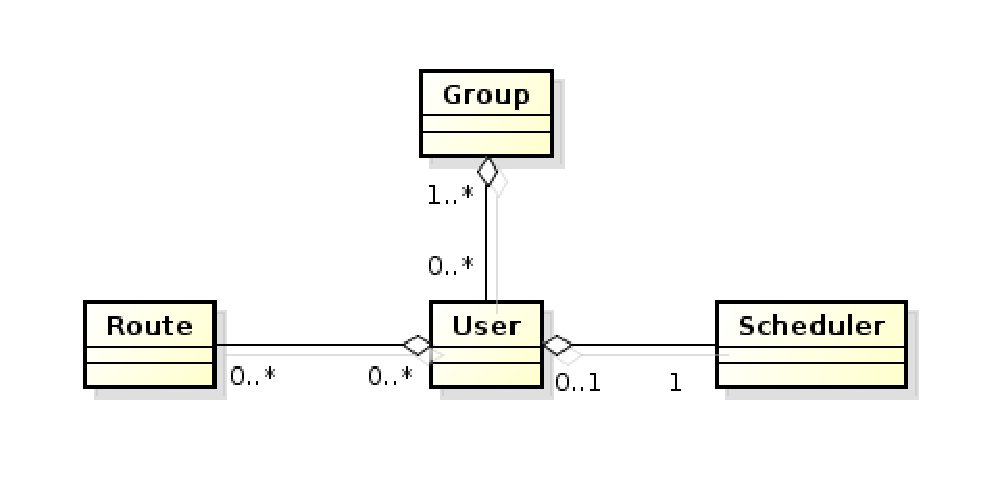
\includegraphics[scale=0.55]{figuras/capitulo5/diagrama_classe.eps}
	\caption{Diagrama de classe inicial}
	\label{diagrama de classe}
\end{figure}

Este modelo servirá como base para a implementação de todas as funcionalidades propostas.

\section{Outros Trabalhos Relacionados}

\section{Resumo do Capítulo}
